\documentclass[12pt,a4paper]{article}
\usepackage{iftex}
\ifPDFTeX
    \usepackage[utf8]{inputenc}
    \usepackage[T1]{fontenc}
    \usepackage{mathpazo} % Palatino font
\else
    \usepackage{fontspec}
    \setmainfont{Times New Roman}
\fi
\usepackage[brazilian]{babel}
\usepackage{amsmath, amssymb, amsthm}
\usepackage[linesnumbered,ruled,vlined,portuguese]{algorithm2e}
\usepackage{listings}
\usepackage{graphicx}
\usepackage{booktabs}
\usepackage{geometry}
\usepackage{float}
\usepackage{xcolor}
\usepackage{setspace}
\usepackage[colorlinks=true, linkcolor=blue, urlcolor=blue, citecolor=blue]{hyperref}

\geometry{margin=2.5cm}
\onehalfspacing

% Colors for code blocks
\definecolor{codebg}{rgb}{0.96,0.96,0.96}
\definecolor{codekey}{rgb}{0.0,0.4,0.8}
\definecolor{codestr}{rgb}{0.6,0.1,0.1}
\definecolor{codecom}{rgb}{0.4,0.6,0.4}

\lstset{
    backgroundcolor=\color{codebg},
    commentstyle=\itshape\color{codecom},
    keywordstyle=\bfseries\color{codekey},
    stringstyle=\color{codestr},
    basicstyle=\ttfamily\footnotesize,
    breaklines=true,
    numbers=left,
    numberstyle=\tiny\color{gray},
    frame=single,
    rulecolor=\color{lightgray},
    captionpos=b,
    tabsize=4
}

\title{
    \vspace{-1cm}
    \begin{center}
        \Large \textbf{Universidade Federal do Ceará -- UFC} \\
        \large Departamento de Computação \\
        \vspace{1cm}
        \Huge \textbf{Métodos Numéricos II} \\
        \vspace{0.5cm}
        \Large \textit{Relatório da Unidade 1: Diferenças Finitas e Processamento Digital de Imagens}
    \end{center}
}
\author{
    Nicolas Wallace Amorim Perote -- Matrícula: 566512 \\
    Samyra Vitória Lima de Almeida -- Matrícula: 521240
}
\date{\today}

\begin{document}

\maketitle
\tableofcontents
\newpage

\section{Introdução}
O presente documento tem como objetivo relatar as implementações e análises desenvolvidas durante a Unidade 1 da disciplina de Métodos Numéricos II. O foco central desta etapa é a exploração das \textbf{diferenças finitas} como principal ferramenta para o cálculo numérico de derivadas. Esta técnica permite avaliar taxas de variação de funções de forma discreta, um requisito fundamental na modelagem computacional onde soluções analíticas são frequentemente indisponíveis.

Além dos conceitos matemáticos puros, o relatório estende a aplicação das derivadas numéricas para o domínio do \textbf{processamento digital de imagens}. Nesse contexto, a imagem é tratada como uma função de duas variáveis espaciais, $I(x,y)$. Os gradientes dessa função revelam flutuações e transições abruptas de brilho, caracterizando os contornos e formas dos objetos presentes na cena.

O relatório apresenta a base teórica, as fórmulas extraídas por expansão de Taylor, a modelagem algorítmica e os testes em ambiente computacional utilizando a linguagem Python e as bibliotecas Numpy e Scipy.

\section{Diferenciação Numérica}
As aproximações de derivadas por meio de computação dependem de avaliações em pontos vizinhos. Para tanto, utilizamos as séries de Taylor em torno de um ponto $x$, com passo $h$.

\subsection{Fundamentação Teórica}
A expansão fundamental da função $f(x+h)$ é dada por:
\begin{equation}
f(x+h) = f(x) + hf'(x) + \frac{h^2}{2}f''(x) + \frac{h^3}{6}f'''(x) + \mathcal{O}(h^4).
\end{equation}
Ao manipularmos essa equação algebricamente e desprezarmos os termos de ordem superior, obtemos os estimadores de diferenças \textit{Forward} (progressivas) e \textit{Backward} (regressivas). Combinando as expansões em $(x+h)$ e $(x-h)$, eliminamos os termos de ordem ímpar do erro, derivando as eficientes fórmulas \textit{Centrais}, que naturalmente atingem o erro $\mathcal{O}(h^2)$ ou superior.

\subsection{Fórmulas Implementadas e Ordem de Erro}
A precisão das derivadas numéricas é delimitada pela ordem do erro de truncamento. Neste projeto, a biblioteca matemática desenvolvida abrange até o erro quártico ($\mathcal{O}(h^4)$). Algumas das equações notáveis utilizadas no código são expostas a seguir.

\subsubsection{Métodos de Alta Precisão (Erro Quártico $\mathcal{O}(h^4)$)}
Para atingir uma convergência mais rápida sem a necessidade de passos $h$ excessivamente diminutos (o que ampliaria erros de arredondamento de ponto flutuante), fórmulas com truncamento $\mathcal{O}(h^4)$ são primordiais.
\begin{itemize}
    \item \textbf{Primeira Derivada Central:}
    \begin{equation}
    f'(x) \approx \frac{-f(x+2h) + 8f(x+h) - 8f(x-h) + f(x-2h)}{12h}
    \end{equation}
    
    \item \textbf{Segunda Derivada Central:}
    \begin{equation}
    f''(x) \approx \frac{-f(x+2h) + 16f(x+h) - 30f(x) + 16f(x-h) - f(x-2h)}{12h^2}
    \end{equation}
\end{itemize}

O código em Python implementou estas regras de forma otimizada usando dicionários de coeficientes para a varredura linear iterativa, tornando o \textit{design} elegante e orientado a objetos, em contraste com a abordagem repetitiva convencional.

\begin{lstlisting}[language=Python, caption={Método encapsulado de diferenças finitas.}]
def _apply_finite_difference(f, x, h, coefs, denom):
    result = sum(weight * f(x + offset * h) for offset, weight in coefs.items())
    return result / denom
\end{lstlisting}

\subsection{Experimentos e Testes}
Os testes automatizados aplicados sobre a função $f(x)=x^2$ no ponto $x=8$ (cujas derivadas analíticas são $f'(8)=16$, $f''(8)=2$, e $f'''(8)=0$) confirmaram o funcionamento da arquitetura proposta. Todas as variantes de cálculo, especialmente o método \textit{Central}, atingiram a precisão máxima permitida pelos tipos de dado \texttt{float64}, exibindo erro prático virtualmente nulo para $h=0.5$.

\section{Filtros e Processamento de Imagens}
No domínio bidimensional de uma matriz de pixels, derivadas são sinônimo de detecção de bordas (edges). A transição de cor representa uma derivada local elevada.

O processamento consistiu em dois algoritmos principais baseados em convolução bidimensional com núcleos (kernels) matemáticos gerados pelas fórmulas derivadas da Seção anterior.

\subsection{Algoritmo 1: Operador Gradiente (Sobel)}
O Algoritmo 1 baseia-se na detecção de picos na primeira derivada da imagem. Utilizou-se um filtro Gaussiano $\mathcal{N}(\mu, \sigma)$ prévio para suavizar a matriz de pixels, minorando ruídos de alta frequência. Em seguida, os operadores de Sobel são aplicados nas direções $x$ e $y$.
Diferentemente do Sobel clássico, nosso kernel foi expandido e refinado para alta precisão utilizando a máscara correspondente à Diferença Central $\mathcal{O}(h^4)$, isto é, $[-1, 8, 0, -8, 1]/12$.

A magnitude do gradiente é definida como $G = \sqrt{G_x^2 + G_y^2}$. A imagem binarizada de saída destaca unicamente pixels com intensidade superior ao limiar \textit{threshold}.

\subsection{Algoritmo 2: Laplaciano da Gaussiana}
O Laplaciano rastreia o cruzamento por zero da segunda derivada. Por se tratar de um operador isotrópico (independente de direção), capta contornos mais complexos e fechados. Matematicamente, ele resolve $\nabla^2 I = \frac{\partial^2 I}{\partial x^2} + \frac{\partial^2 I}{\partial y^2}$.

Implementamos um kernel 5x5 de alta fidelidade montado a partir da matriz $1D$ de segunda derivada $\mathcal{O}(h^4)$ e convolvemos o espaço de busca mediante as diretivas avançadas do \texttt{scipy.signal.convolve2d}.

\subsection{Resultados Visuais}
A fim de verificar a resposta algorítmica, o código \texttt{processamento\_imagens.py} processa uma matriz sintética $10 \times 10$ controlada, seguido do mapeamento na fotografia real (Batman.jpg).

\begin{figure}[H]
    \centering
    \begin{minipage}{0.48\textwidth}
        \centering
        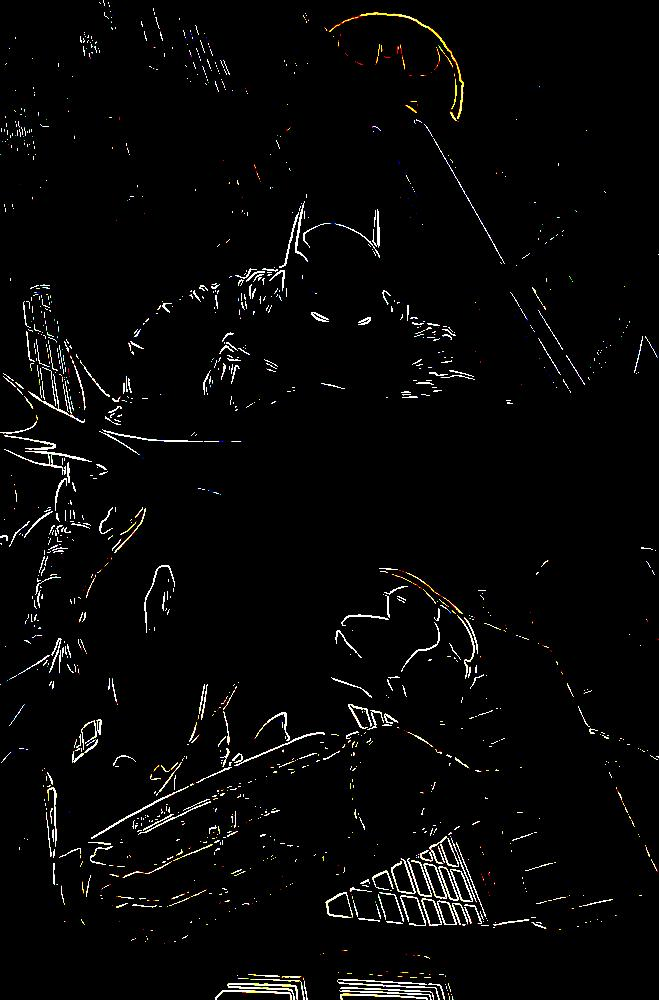
\includegraphics[width=\textwidth]{batman_sobel_refat.jpg}
        \caption{Imagem processada via Algoritmo 1 (Sobel)}
    \end{minipage}\hfill
    \begin{minipage}{0.48\textwidth}
        \centering
        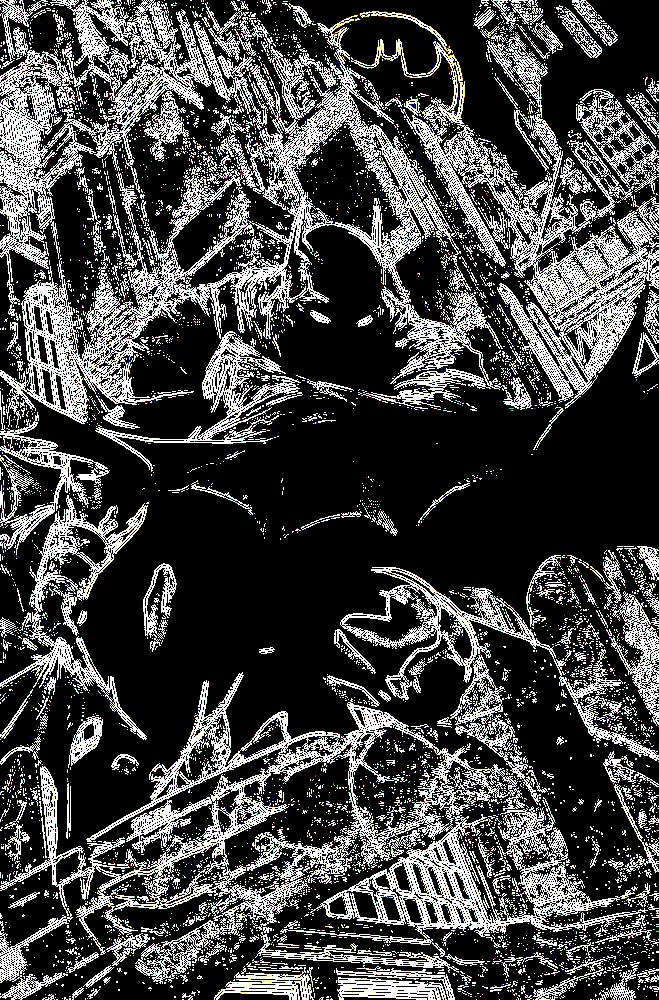
\includegraphics[width=\textwidth]{batman_laplace_refat.jpg}
        \caption{Imagem processada via Algoritmo 2 (Laplace)}
    \end{minipage}
\end{figure}

Observa-se que o método de Sobel produz contornos direcionais grossos e persistentes. Já a malha formada pelo Laplaciano exibe contornos agudos, sensíveis a detalhes sutis (frequências médias), revelando arestas finas e bem demarcadas, mas com propensão natural a ruído devido à amplificação provocada pela derivada secundária.

\section{Considerações Finais}
A elaboração da Unidade 1 ratificou de forma pragmática que a matemática discreta atua como pilar elementar de diversas ferramentas tecnológicas modernas. Através da conversão do cálculo diferencial contínuo para equações de somatórias e limites numéricos, construímos um ferramental robusto capaz de extrair informações semânticas relevantes de matrizes imagéticas. 

A refatoração do código com o ecossistema \texttt{NumPy/SciPy} também elevou de forma drástica a eficiência temporal, utilizando vetorialização subjacente em C ao invés de laços (\textit{for loops}) em matrizes nativas do Python. Essa modernização do projeto não apenas reduziu o custo computacional, mas abriu portas para um \textit{design pattern} de altíssimo escalonamento.

\end{document}
